\documentclass[10pt,twocolumn,letterpaper]{article}

\usepackage{cvpr}
\usepackage{times}
\usepackage{epsfig}
\usepackage{graphicx}
\usepackage{amsmath}
\usepackage{amssymb}

% Include other packages here, before hyperref.

% If you comment hyperref and then uncomment it, you should delete
% egpaper.aux before re-running latex.  (Or just hit 'q' on the first latex
% run, let it finish, and you should be clear).
\usepackage[breaklinks=true,bookmarks=false]{hyperref}

\cvprfinalcopy % *** Uncomment this line for the final submission

\def\cvprPaperID{****} % *** Enter the CVPR Paper ID here
\def\httilde{\mbox{\tt\raisebox{-.5ex}{\symbol{126}}}}

% Pages are numbered in submission mode, and unnumbered in camera-ready
%\ifcvprfinal\pagestyle{empty}\fi
\setcounter{page}{4321}
\begin{document}

%%%%%%%%% TITLE
\title{Project: Your TITLE goes here}

\author{First Author\\
{\tt\small firstauthor@i1.org}
% For a paper whose authors are all at the same institution,
% omit the following lines up until the closing ``}''.
% Additional authors and addresses can be added with ``\and'',
% just like the second author.
% To save space, use either the email address or home page, not both
\and
Second Author\\
{\tt\small secondauthor@i2.org}
}

\maketitle
%\thispagestyle{empty}

%%%%%%%%% ABSTRACT
\begin{abstract}
   In the abstract, you should describe in a few sentences the problem you are solving and which method you are using to do so. An abstract should give a reader that is already familiar with the topic a general idea what the paper is about. 
\end{abstract}

%%%%%%%%% BODY TEXT
\section{Introduction}
The introduction can be seen as an explanation for readers that are not that familiar with the topic. First, you shortly motivate the topic your are trying to solve. Afterwards, you give a rough idea how your method solves the problem. 


%-------------------------------------------------------------------------
\section{Related Work}
Usually, the related work section lists and introduces literature about the problem that has already been published or on similar methods applied to other problems. In your case, it is fine to list the literature you gain your information from. Literature you refer to has to be included in the file "literature.bib". You can cite it by \cite{ren2015faster}.

\section{Method}
In this section, you should describe the method you used to solve the problem in detail. Figures can help to explain the used method. An example how to insert a figure is given in Figure \ref{fig:long}. \\
Also, formulas often help to make the mathematical background clearer. How to insert them is given here: 
$$a + b + a = 2 \cdot a + b\,.$$
It is essential that the reader is able to understand your method according to this section.

\begin{figure}[t]
	\begin{center}
		%\fbox{\rule{0pt}{2in} \rule{0.9\linewidth}{0pt}}
		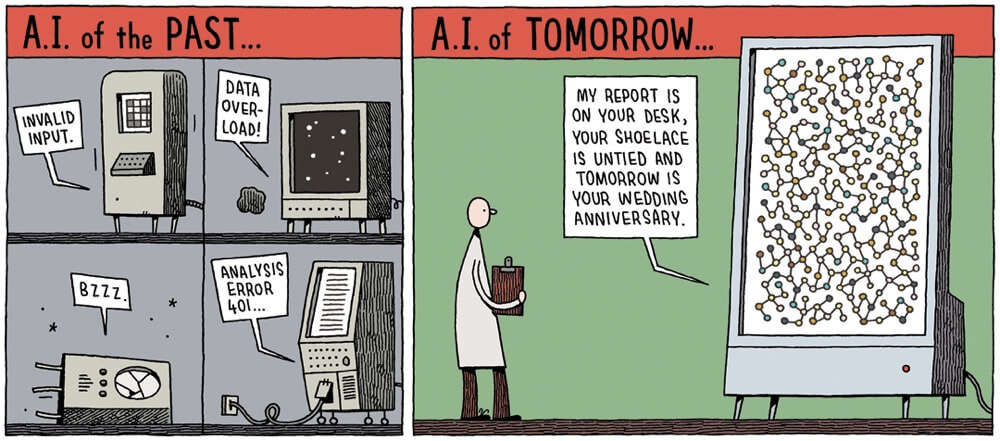
\includegraphics[width=1.0\linewidth]{AI-comic-funny.jpg}
	\end{center}
	\caption{Overview of method/ Network structure}
	\label{fig:long}
\end{figure}

\section{Evaluation}
\subsection{Experimental Setup}
Here, you should describe the data you used for training, the hyper parameter settings, how you split the data into a training and a test set, etc.. Additionally, you should explain how you adapted your method to work well on your problem setup.




\subsection{Discussion}
In the discussion, you present and discuss the results your method achieved in the provided setups, why which set up works better, ... . The numbers (accuracy of your TEST set) should be given in a table, as e.g. Table \ref{tab:results}. You should also show exemplary images for which you achieved good results and examples, where the algorithm did not work as expected. Give possible explanations for both cases, e.g. ``what could be the reason for missing a Pedestrian? ``.

\begin{table}
	\begin{center}
		\begin{tabular}{|l|c|}
			\hline
			Method & Frobnability \\
			\hline\hline
			Theirs & Frumpy \\
			Ours & Makes one's heart Frob\\
			\hline
		\end{tabular}
	\end{center}
	\caption{Results. Ours is better.}
	\label{tab:results}
\end{table}

\section{Conclusion and Future Work}
Finally, you shortly summarize what you achieved in your work and point out what could be done in the future to get even better results. 









%-------------------------------------------------------------------------

{\small
\bibliographystyle{ieee_fullname}
\bibliography{literature}
}

\end{document}
